% SO(2) como rotaciones en el círculo
% Compilar con: pdflatex so2_rotations.tex
\documentclass[tikz,border=10pt]{standalone}
\usepackage{tikz}
\usepackage{amsmath}
\usetikzlibrary{arrows.meta, calc, decorations.markings}

\definecolor{gdlblue}{RGB}{41, 98, 168}
\definecolor{gdlred}{RGB}{191, 49, 49}
\definecolor{gdlgreen}{RGB}{30, 130, 76}
\definecolor{gdlorange}{RGB}{217, 130, 30}
\definecolor{gdlpurple}{RGB}{118, 56, 138}
\definecolor{gdlgray}{RGB}{140, 140, 140}
\definecolor{gdlyellow}{RGB}{190, 140, 10}

\begin{document}
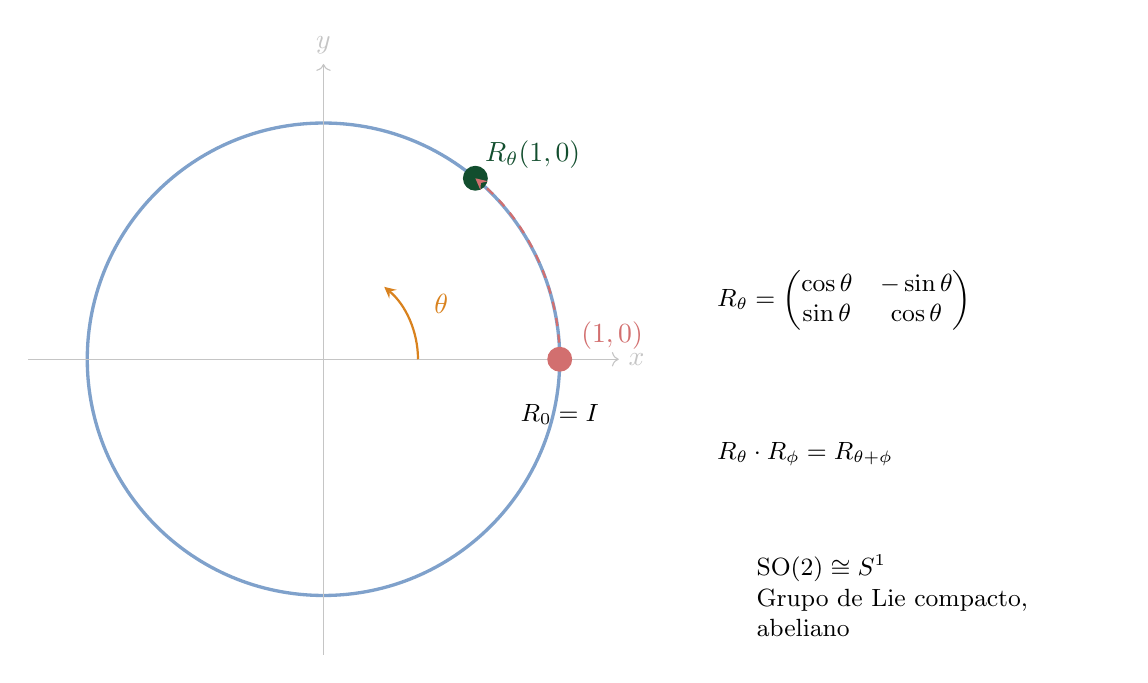
\begin{tikzpicture}[scale=1.5]

% Círculo principal S¹
\draw[very thick, gdlblue!60] (0,0) circle (2cm);

% Ejes
\draw[gdlgray!50, ->] (-2.5,0) -- (2.5,0) node[right] {$x$};
\draw[gdlgray!50, ->] (0,-2.5) -- (0,2.5) node[above] {$y$};

% Punto inicial (1,0)
\fill[gdlred!70] (2,0) circle (3pt);
\node[right, gdlred!70] at (2.1,0.2) {$(1,0)$};

% Rotación por ángulo θ
\def\angle{50}
\coordinate (rotated) at ({2*cos(\angle)}, {2*sin(\angle)});
\fill[gdlgreen!60!black] (rotated) circle (3pt);
\node[above right, gdlgreen!60!black] at (rotated) {$R_\theta(1,0)$};

% Arco de ángulo
\draw[thick, gdlorange, ->, >=stealth] (0.8,0) arc (0:\angle:0.8cm);
\node[gdlorange] at ({1.1*cos(\angle/2)}, {1.1*sin(\angle/2)}) {$\theta$};

% Flecha de rotación
\draw[thick, gdlred!70, ->, >=stealth, dashed] (2,0) arc (0:\angle:2cm);

% Matriz de rotación
\node[font=\small, text width=5cm] at (5, 0.5) {
    $R_\theta = \begin{pmatrix} \cos\theta & -\sin\theta \\ \sin\theta & \cos\theta \end{pmatrix}$
};

% Propiedad del grupo
\node[font=\small, text width=5cm] at (5, -0.8) {
    $R_\theta \cdot R_\phi = R_{\theta + \phi}$
};

% Círculo como grupo
\node[font=\small, text width=4cm] at (5, -2) {
    $\mathrm{SO}(2) \cong S^1$\\
    Grupo de Lie compacto, abeliano
};

% Etiqueta de identidad
\node[below, font=\small] at (2,-0.3) {$R_0 = I$};

\end{tikzpicture}
\end{document}
